%!TEX root = ../thesis.tex
\chapter{Introduction}
\label{introduction}

\hl{introduzione a significato di way of working (in SW)
	cercare articoli da blog per spiegare
	martin fowler		

fare tracking delle isssue / bug è diventato difficile / complesso
	molti tool open source che fanno anche documentazione e code review (altri aspetti)

l'evoluzione negli ultimi anni nelle aziende IT
	necessità di organizzazione delle azienda e la necessità di avere una gerarchia (o simil gerarchia)

ho sperimentato questo approccio in athonet, mostrata interessata all'utilizzo di un gestionale sw di tipo agile per la gestione dei processi di sviluppo sw interni

I have sperimented ... 
}

\section{Premise}

	This document represents a report of the two month curricular internship done between June and July 2019 at Athonet under the supervision of Dr. Fabio Giust.
	It contains a description of the work that I have done and an introduction to Agile and Scrum software developing methodologies.
	To introduce or to describe some of the arguments I will be using some comic strips of Dilbert, a character invented by Scott Adams.
	It satirically represents the problems that can be present in a small or big company of software development.
	
	\begin{figure}[H]
		\centering
		
\includegraphics[width=1\textwidth]{resources/Dissertate}\\
		\caption{The issues related with Jira and Confluence are handled by a dedicated Jira Cloud instance}
	\end{figure}
	
\section{The company}

	Athonet is a telecommunication company headquartered nearby Vicenza.
	It was born from the idea that broadband networking should be easier to access and more available for people in rural areas and for companies that work in mission critical services or special environments like shipping, mining companies or even hospitals (safety critical).
	Officially it was started in 2004, although a working prototype was already developed by the CEO and CTO that were working alongside in Ericson at that time.
	\begin{figure}[H]
		\centering
		
\includegraphics[width=.7\textwidth]{resources/ath_logo}\\
		\caption{Athonet's logo}
	\end{figure}
	Low latency communication, reliability and security are at the core of what Athonet provides.
	Their main product is PriMo, a device that allows to create a dedicated core network, or enterprise LTE.
	\begin{figure}[H]
		\centering
		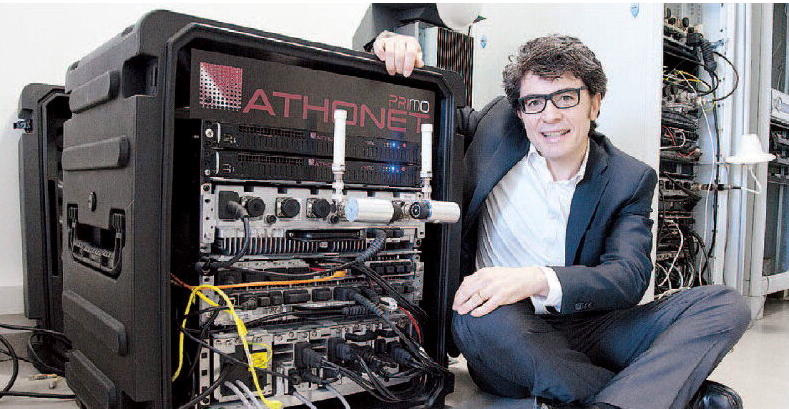
\includegraphics[width=.7\textwidth]{resources/gianluca_primo}\\
		\caption{The CTO, \textit{Gianluca Verin}, with Athonet's main product \textbf{\textit{PriMo}}}
	\end{figure}
	They showed how this product performs in an emergency situation on the field in Emilia Romagna, when in 2012, after the disastrous earthquake has destroyed all the communication lines Athonet has reestablished communications.
	Athonet arrived with PriMo and installed it at the top of a school, allowing them to cover the affected area not only for the operators of Servizio Civile but for the citizens as well.
	In December 2013, Athonet, along other companies, has been rewarded by Giorgio Napolitano, the then President of the Italian Republic, with a medal for merits for the sustainability in the digital sector.
%	meriti nel settore del digitale per la sostenibilità
	Lately they have migrated some of their functions to the cloud: by using AWS they have achieved a hybrid product, BubbleCloud, a plug and play solution that allows to locally deploy the physical Edge Nodes while managing them from the AWS cloud.
	This company may still be small but has much to offer, considering that some of it's competitors are giants like Nokia and Ericson.
	Athonet's passion and dedication are demonstrated through the awards and prizes that has won, for example this year, 2019, has won a total of 4 Global Mobile Awards including CTO’s choice at the GSMA in Barcellona.
%	https://www.millionaire.it/athonet-la-startup-italiana-che-trionfa-al-mobile-world-congress/#!
%	http://www.ilgiornale.it/news/interni/genio-torna-svezia-soffrire-nella-sua-italia-912407.html

\section{The project}

	I have chosen to do my internship at Athonet because the project, although may seem simple, is quite interesting.
	It consists in installing and configuring two main software tools, Jira and Confluence, alongside plugins to add more functions and enhance their potentiality.
	However, the most important part of this project is not installing the software, but adapting it to the needs of the company.
	As said earlier Athonet my still be small, but it's a growing company, and because of this it needs to give itself some internal rules and specifications to follow when working on a task, communicating with the client or even share internal information to employees.
	Not only for themselves but for clients they work with as well, since most big companies require that their partners have internal regulations, no matter the number of people in the company.
	As I will explain in the following chapters Jira is an Issue Tracking System, a software that allows to follow the tasks (like resolving bugs or implementing features) that are related to a project, while Confluence is a software for sharing knowledge, that means sharing internal documents, keeping a wiki, having documentation available and even for customers.
	My task was to demonstrate that these tools are what Athonet needs to be a strong an coherent company, where information is always shared and available, while maintaining a history of changes, by creating an environment that suited their needs and that can evolve alongside the company.
	To do this I have learned the basics of Agile and Scrum methodologies, how a company operates internally and with their clients and how introducing a new tool may improve the way of working, even if it creates chaos at the beginning.

\section{Document organization}
	This document is organized as follows:
	\begin{itemize}
		\item Chapter 1 or \textit{Introduction}: describes the overall content of this document
		\item Chapter 2 or \textit{The internship project}: describes in detail the objectives and planning of the internship project
		\item Chapter 3 or \textit{Agile processes and methodologies}: an introduction to the Agile software development
		\item Chapter 4 or \textit{Jira and Confluence: the essentials}: describes the most valuable functionalities of Jira and Confluence
		\item Chapter 5 or \textit{Project implementation}: details how the project has been implemented by dividing it into time periods
		\item Chapter 6 or \textit{Conclusions}: contains the retrospective of the project, future developments and personal considerations
	\end{itemize}
